\section{Thesis Plan}
In this section of the report, I discuss my thesis plan. As per my plan, I have three contributory chapters in my thesis. These chapters are as follows.

\subsection{Chapter-1: Study on Online Video Streaming System}
In this chapter, we will present out study on the most popular video streaming platform YouTube. We study the adaptation system and the transport protocol used by YouTube. Our study found that YouTube's video quality strongly correlated with the remaining buffer in the video player. It tries to maintain an optimal buffer length, and if it fails to do so, it drops the quality. However, it does not drop the quality immediately. Instead, it tries to download a smaller segment if possible. The ACM NOSSDAV 2017 conference published this work.

We also found that YouTube (and the entire Google services) started using a new transport protocol QUIC. So, we start analyzing the performance of QUIC protocol on video streaming. However, we could not continue the work efficiently as we do not have any control over the streaming server. We perform a similar set of experiments using an openly available DASH-IF video streaming system and found that QUIC does not perform well in terms of video quality. I have a published paper on this work in the IEEE networking letter.

\subsection{Chapter-2: Mobility Aware Energy-Efficient Video Streaming System}
After studying YouTube and DASH based streaming system, we find that there is a problem with video streaming and energy requirements. So, we start pilot studies to understand the power consumption by different network conditions. We have the work in detail in this report. The work is published in the IFIP Networking 2020 conference.

\subsection{Chapter-3: Coalition Based Federated Live Streaming System}
Live video streaming is becoming an alternative to the television system. More and more users are watching live streaming; many users belong to the same local area network sharing a single Internet connection. We developed a system called FliDASH to form a coalition among the player from a local area network so that a segment needs to be downloaded by only one player in a coalition. The experimental results show that the FliDASH improves QoE and video quality for each and every player in the system and significantly reduces the server load. It is published in ACM SIGCOMM NAI 2020.

\subsection{Requirement of the extension}
Among these chapters, we are working on an extension of chapter 2. Once it is done, we are planning to submit the extension work to a journal. Thus I need an extension. Fig.~\ref{fig:pendingtask} describe the pending tasks with expected completion time.
 \begin{figure}[h]
	\centering
	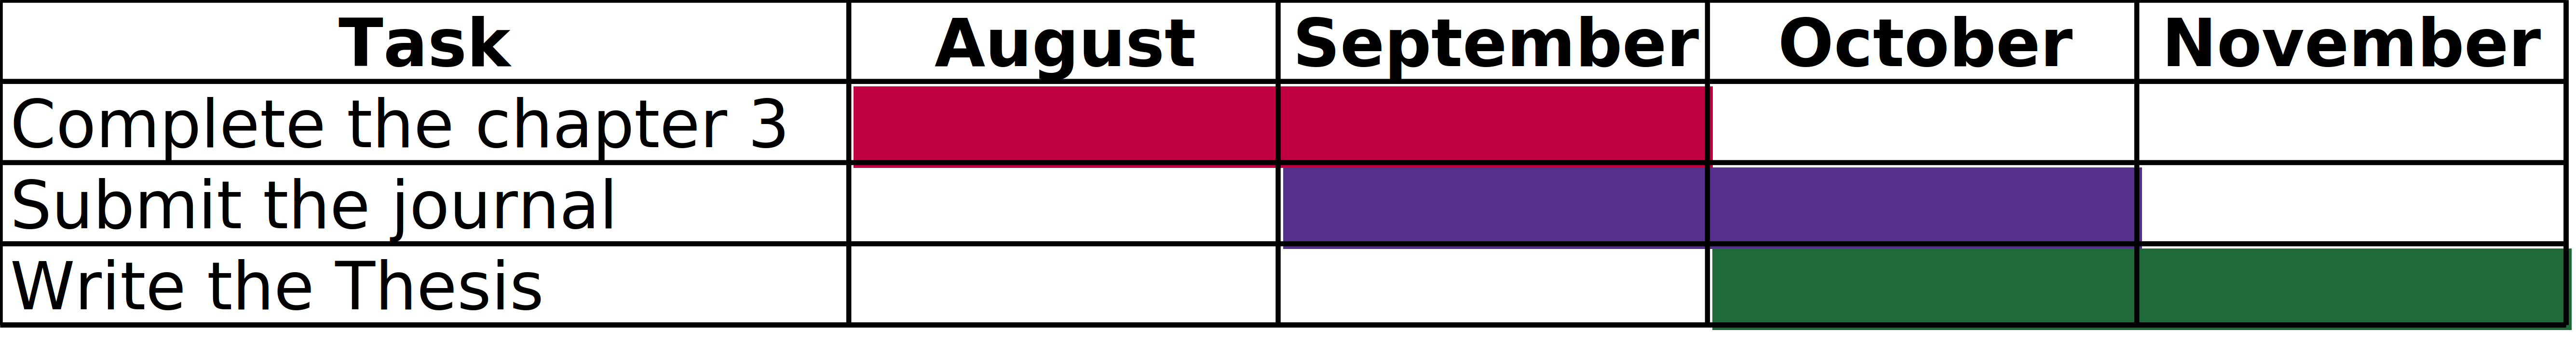
\includegraphics[width = 0.7\textwidth]{figures/chart}
	\caption{The pending tasks and expected completion time}
	\label{fig:pendingtask}
\end{figure}

\section*{Publications}
\begin{enumerate}[start=1,label={[\arabic*]}]
	\item \textbf{Abhijit Mondal}, Sandip Chakraborty, ``\textit{Federated Adaptive Bitrate Live Streaming over Locality Sensitive Playback Coalitions}”, in the Proceedings of the Workshop on Network Application Integration/CoDesign (NAI '20), Association for Computing Machinery, New York, USA, August 11 - 14, 2020. 
	\item \textbf{Abhijit Mondal}, Sandip Chakraborty, ``\textit{Does QUIC Suit Well with Modern Adaptive Bitrate Streaming Techniques?}”, in IEEE Networking Letters, vol. 2, no. 2, pp. 85-89, June 2020.
	\item \textbf{Abhijit Mondal}, Basabdatta Palit, Somesh Khandelia, Nibir Pal, Jay Jayatheerthan, Krishna Paul, Niloy Ganguly and Sandip Chakraborty, ``\textit{EnDASH - A Mobility Adapted Energy Efficient ABR Video Streaming for Cellular Networks}'', in the Proceedings of 2020 IFIP Networking Conference (IFIP Networking), Paris, France, June 22-25, 2020.
	\item \textbf{Abhijit Mondal}, Satadal Sengupta, B.R. Reddy, M.J.V. Koundinya, Chander G., Pradipta De, Niloy Ganguly, Sandip Chakraborty, ``\textit{Candid with YouTube: Adaptive Streaming Behavior and Implications on Data Consumption}'' in Proceedings of the 27th Workshop on Network and Operating Systems Support for Digital Audio and Video (ACM NOSSDAV’17), Taipei, Taiwan, June 20 - 23, 2017.
\end{enumerate}